\documentclass[12pt]{report}

\usepackage{fullpage}
\usepackage{fancyhdr}
\usepackage{url}
\usepackage{color, colortbl}
\definecolor{green}{rgb}{0,1,0}
\usepackage{tabularx,ragged2e,booktabs,caption}
\usepackage{graphicx}

\newcommand{\BibTeX}{{\sc Bib}\TeX}

%%%%%%%%%%%%%%%%%%%%%%%%%%%%%%%%%%%%%%%%%%%%%
%%%%%%				PAGE NUMBERING					       %%%%%%
%%%%%%%%%%%%%%%%%%%%%%%%%%%%%%%%%%%%%%%%%%%%%

\pagestyle{fancy}

\lhead{}
\chead{}
\rhead{\thepage}
\lfoot{}
\cfoot{}
\rfoot{}
\renewcommand{\headrulewidth}{0 pt}
\renewcommand{\footrulewidth}{0 pt}

%%%%%%%%%%%%%%%%%%%%%%%%%%%%%%%%%%%%%%%%%%%%%
%%%%%%				START OF DOCUMENT				       %%%%%%
%%%%%%%%%%%%%%%%%%%%%%%%%%%%%%%%%%%%%%%%%%%%%

\begin{document}

%%%%%%%%%%%%%%%%%%%%%%%%%%%%%%%%%%%%%%%%%%%%%
%%%%%%				TITLE PAGE						       %%%%%%
%%%%%%%%%%%%%%%%%%%%%%%%%%%%%%%%%%%%%%%%%%%%%

\noindent Team \#4 \\  \\
Project \#28: LogicBlockz \\ \\
Stephen Coombes \\
Ryan Hart \\
David Tyler \\ \\
Capstone Proposal \\ \\
\today \\ \\ \\ \\ \\
\centerline{Requirements and Solution Report}
\newpage

%%%%%%%%%%%%%%%%%%%%%%%%%%%%%%%%%%%%%%%%%%%%%
%%%%%%				END TITLE						       %%%%%%
%%%%%%				START DOCUMENT					       %%%%%%
%%%%%%%%%%%%%%%%%%%%%%%%%%%%%%%%%%%%%%%%%%%%%

\section*{Introduction}

This document describes the objectives of the capstone project being done by Team \# 4. Our project is an educational puzzle that will teach children the basics of discrete logic and logic gates. We are doing this project because we feel strongly that logic is a good way to introduce children to engineering and computers and that the concepts are simple enough for anyone to learn. We are disappointed this subject was not introduced to us until college, and aim to provide a tool that will increase the exposure of discrete logic to middle and high school students.

\section*{Client Background}

The client for this project is us: Ryan Hart, Stephen Coombes, and David Tyler. We all have an interest in developing an educational, marketable product to both act as a great capstone project as well as possibly make some money after graduation. Our budget for this project is limited to a few hundred dollars, but additional funding can be found upon critical need.

\section*{Problem Statement}

As noted in the introduction, digital logic is not introduced until college, by which point a student has already chosen their field of study.  Younger students are not given an introduction to digital logic and design at an earlier age. 

\section*{Project Objectives}

The goal is to create a hands-on puzzle that will teach children ages 12-18 the basics of logic gates and logic design.  This puzzle toy must also be reasonably priced to encourage widespread adoption.  

\section*{Research Summary}

The major reason we chose to do this project was that we could find no product that does what we are trying to accomplish. However, a couple devices performing fairly similar functions were found.

The most interesting product we found during research was the LogicBlocks Kit \cite{1}. This is basically a do-it-yourself kit that provides small printed circuit boards each containing one logic gate. The circuit boards can be plugged into each other using header pins. The kit provides input, gate, and power blocks. Each gate circuit has an LED on the output to show the logic level. This kit appears appealing to tinker with, but it seems to be geared towards a hobbyist who already has a basic understanding of logic as it does not have a puzzle to solve or any objective. The whole thing is run on a button battery.

The other logic design products we found were mostly computer based. We were already familiar with Logicworks, a logic design software package for engineers \cite{2}. This software was created for professionals and students to design discrete logic circuits. To use it, one essentially draws the schematic on screen and then runs a simulation of the circuit. This software is excellent for aspiring engineers to learn to intricacies of logic design, but most children would get lost in the amount of detail provided. Nevertheless, this software provides some interesting features such as a logic analyzer that we could use in our project.

Another example of a software product is a computer game that challenges the player to solve logic puzzles by designing semiconductors called Kohctpytop \cite{3}. This game is too hard and complex to serve as an introduction to logic, but provides some interesting puzzles, which might be altered to be in our product. Also the angle of semiconductor fabrication is an extremely interesting one. Maybe our product can include some hints as to the underlying operation of the logic gates beyond teaching simply what they do.

\section*{Requirements}

The device shall:
\begin{itemize}

\item Demonstrate the basics of logic design to children aged twelve and up
\item Run on battery power for at least four hours
\item Be a toy
\item Be able to provide time-variant puzzles

\end{itemize}

\noindent The device shall not:
\begin{itemize}

\item In any way represent a hazard to persons in the room

\end{itemize}

\section*{Potential Solutions}

\begin{enumerate}

\item The first solution is to link tiles together via small cables, such as USB cables (which are cheap and widely available).  These cables would be able to provide signal and power connections, and the flexibility of cables prevents any complications of angling tiles.  On the downside, it creates a less-than-elegant solution.
\item The second solution is to link tiles together via physical connectors, e.g. male/female connector ends.  Like USB cables, this can provide signal and power through single connections, but it could lead to fitment concerns.  On the upside, it is sleeker than having an array of cables spilling around, and there are no cables to lose. 
\item The third solution is to build a rigid snap board, with connectors through the bottom of each tile.  The path of the tiles would be defined by the board itself.
\item The fourth solution is to run a daisy-chain of wireless communications and inductive power.  This is the most elegant and technologically advanced concept, however, the net power efficiency on a simple ten block array is under 30\%.
\item The fifth solution is to use an inductive power mat beneath all the blocks, which eliminates cascading inefficiencies.  This solution would also necessitate wireless communication of the signal, and thus it remains a very elegant and sleek solution.  

\end{enumerate}

\section*{Chosen Solution}

\subsection*{Metric}

% Start Metric

\begin{minipage}{\linewidth}
\centering
\captionof{table}{Grabber Mechanism Metric} \label{tab:grabber} 
\begin{tabular}{|l|l|l|l|l|l|l|l|}
\hline
 & Cost & Reliability & Ease Use & Expansion & Replace & Efficiency & Total \\
 \hline
 \rowcolor{green}
Cables & 4 & 4 & 3 & 4 & 4 & 5 & 3.8 \\
Hard Link & 4 & 4 & 2 & 4 & 4 & 5 & 3.6 \\
Snap Grid & 2 & 3.5 & 1 & 0 & 1 & 5 & 2.25 \\
Daisy-Chain & 1 & 2 & 4 & 3 & 2 & 0 & 2.0 \\
Mat & 2 & 3 & 3 & 2 & 1 & 3 & 2.5 \\
Weights & 0.35 & 0.30 & 0.20 & 0.05 & 0.05 & 0.05 & 1.0 \\
\hline
\end{tabular}
\end{minipage}

% End Metric

\subsection*{Explaination}

The daisy chain solution is not viable due to its severe inefficiency, despite the desirable characteristics of creating an exceptionally futuristic design.  The daisy chain shares, to a greater extent, the problem that eliminates the power mat design, in that it is very costly.  This cost concern is largely responsible for the elimination of the power mat design from consideration.  The rigid snap board suffers from poor expansion and lack of creativity possible.  Thus the consideration comes down to hard links versus the cables, and the cables take a slight edge due to the simplicity of connecting cables in any imaginable configuration.  
\newpage
\section*{Schedule}

\begin{figure}[h!]
\begin{center}
	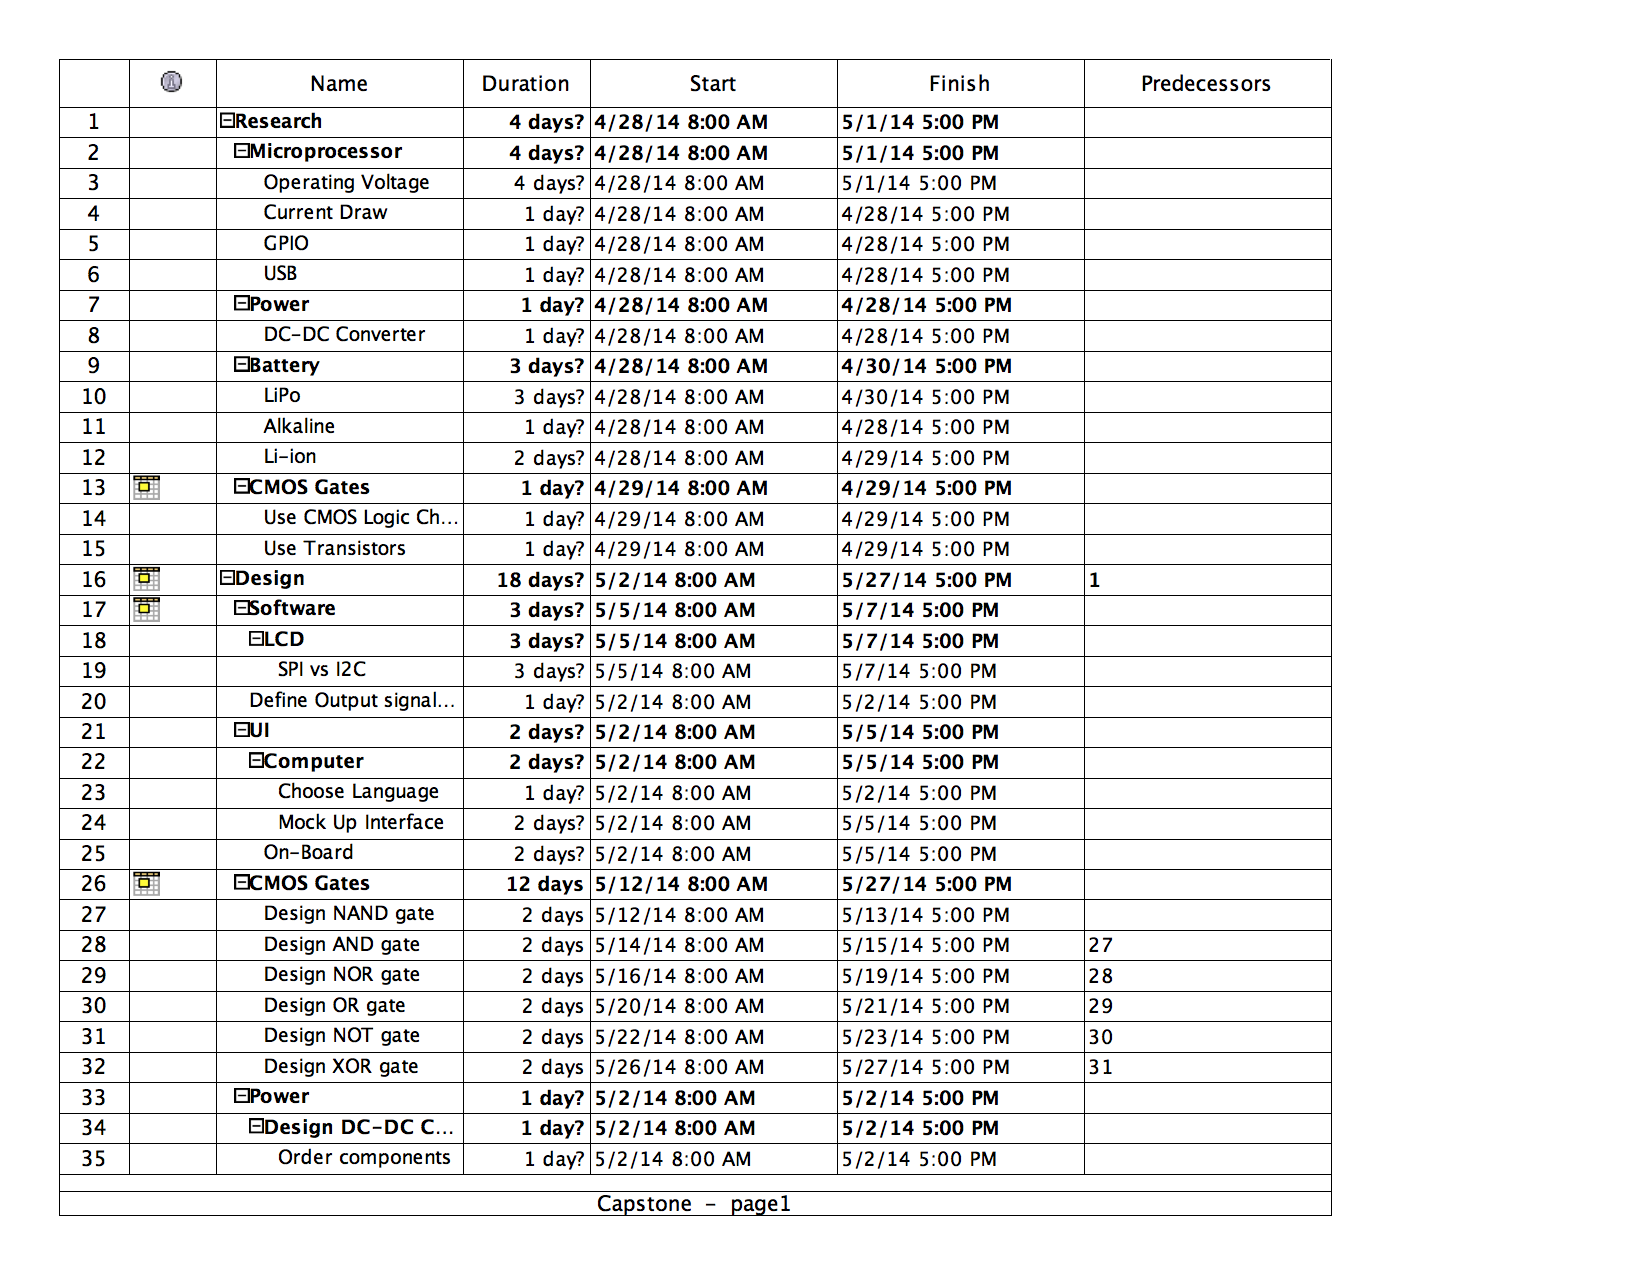
\includegraphics[width=\textwidth]{Schedule}
\label{default}
\end{center}
\end{figure}

\newpage
\begin{figure}[h!]
\begin{center}
	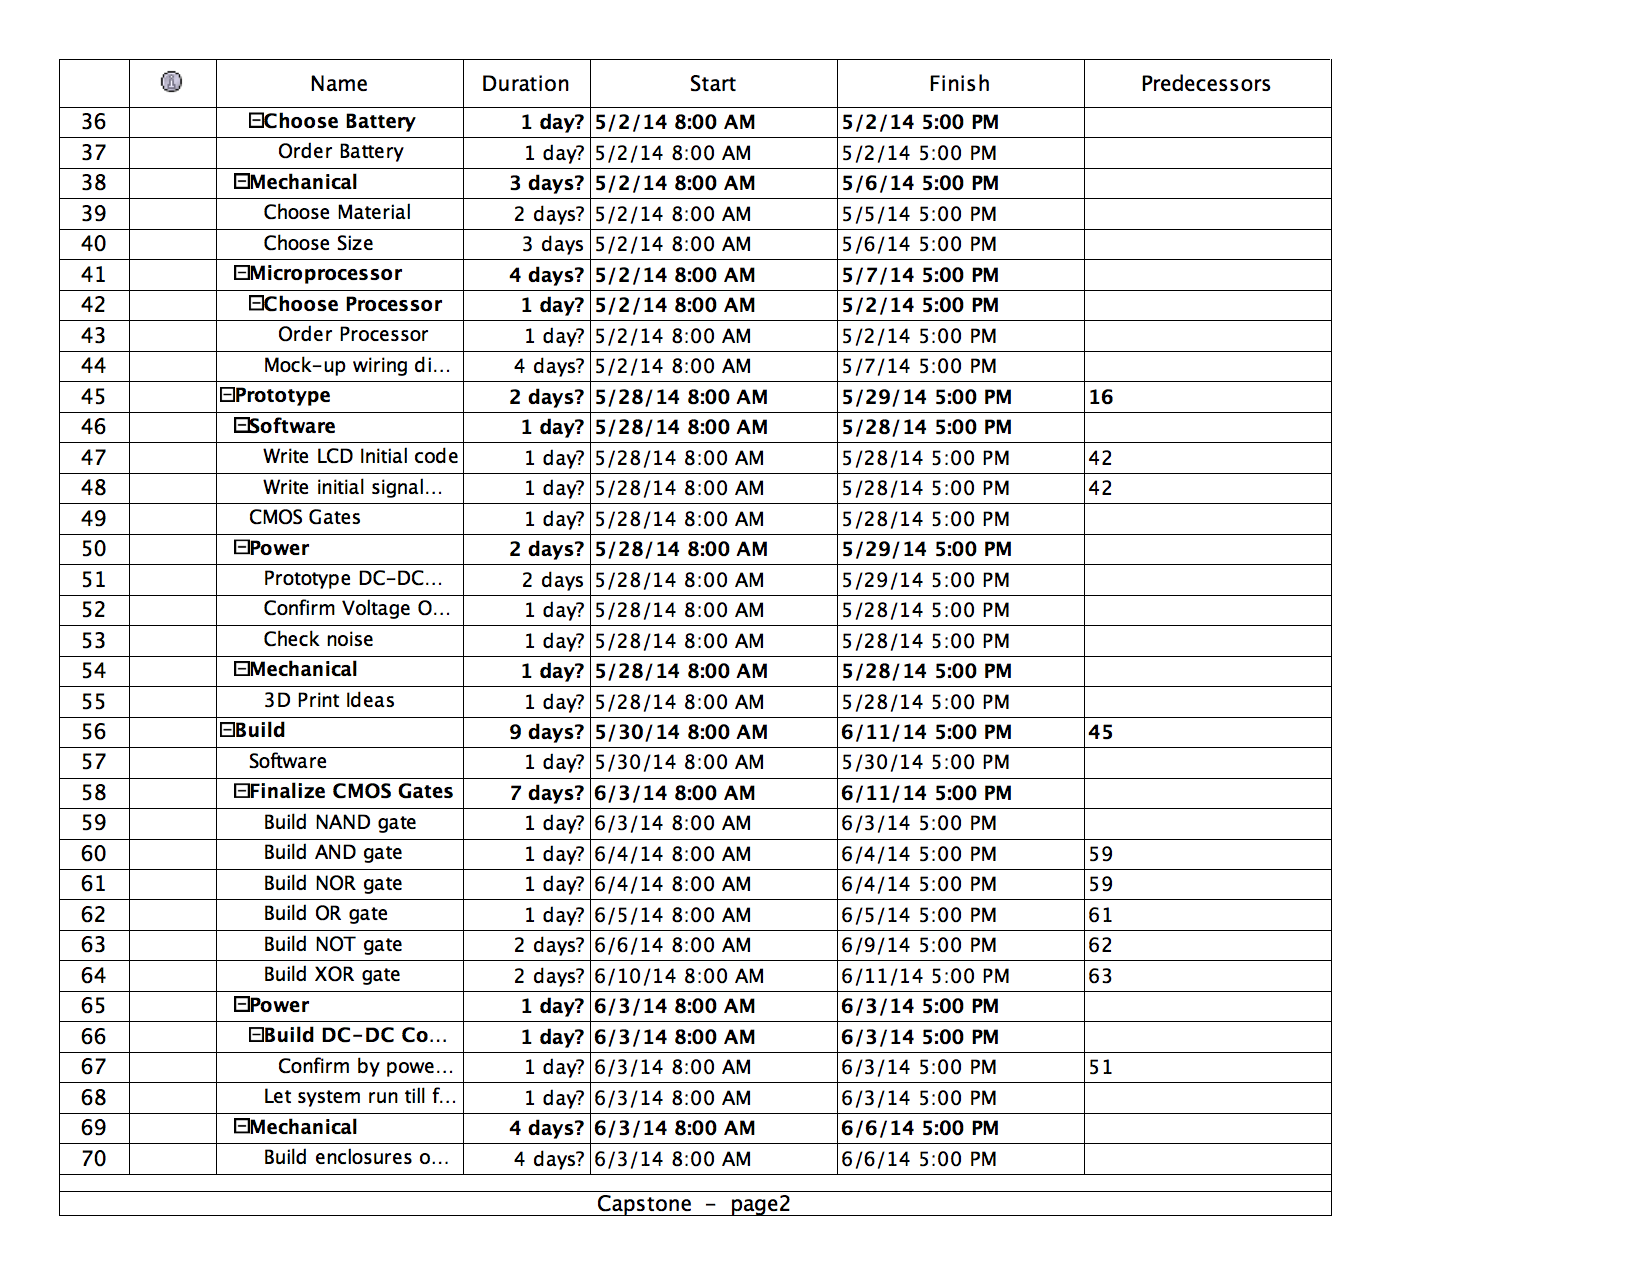
\includegraphics[width=\textwidth]{Schedule2}
\label{default}
\end{center}
\end{figure}

\newpage
\begin{figure}[h!]
\begin{center}
	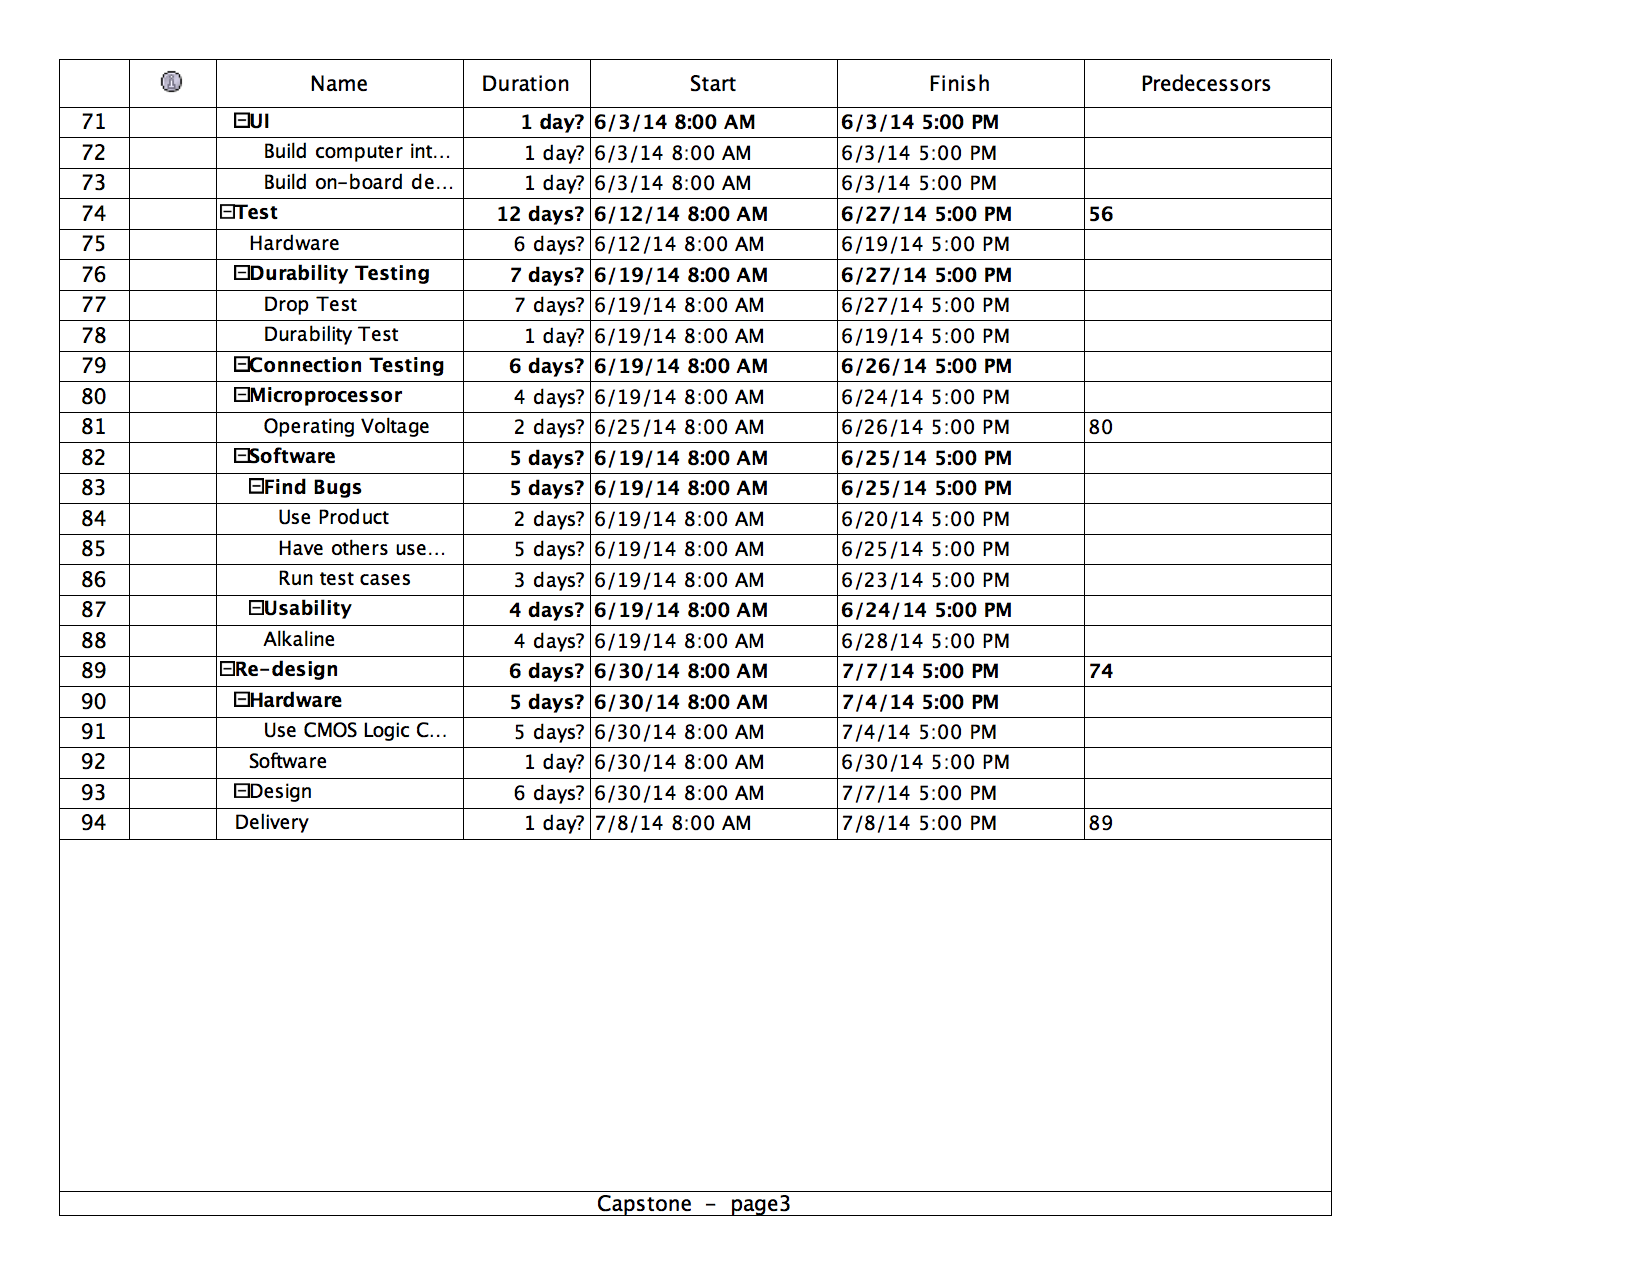
\includegraphics[width=\textwidth]{Schedule3}
\label{default}
\end{center}
\end{figure}


\newpage
\section*{Gantt Chart}

\begin{figure}[h!]
\begin{center}
	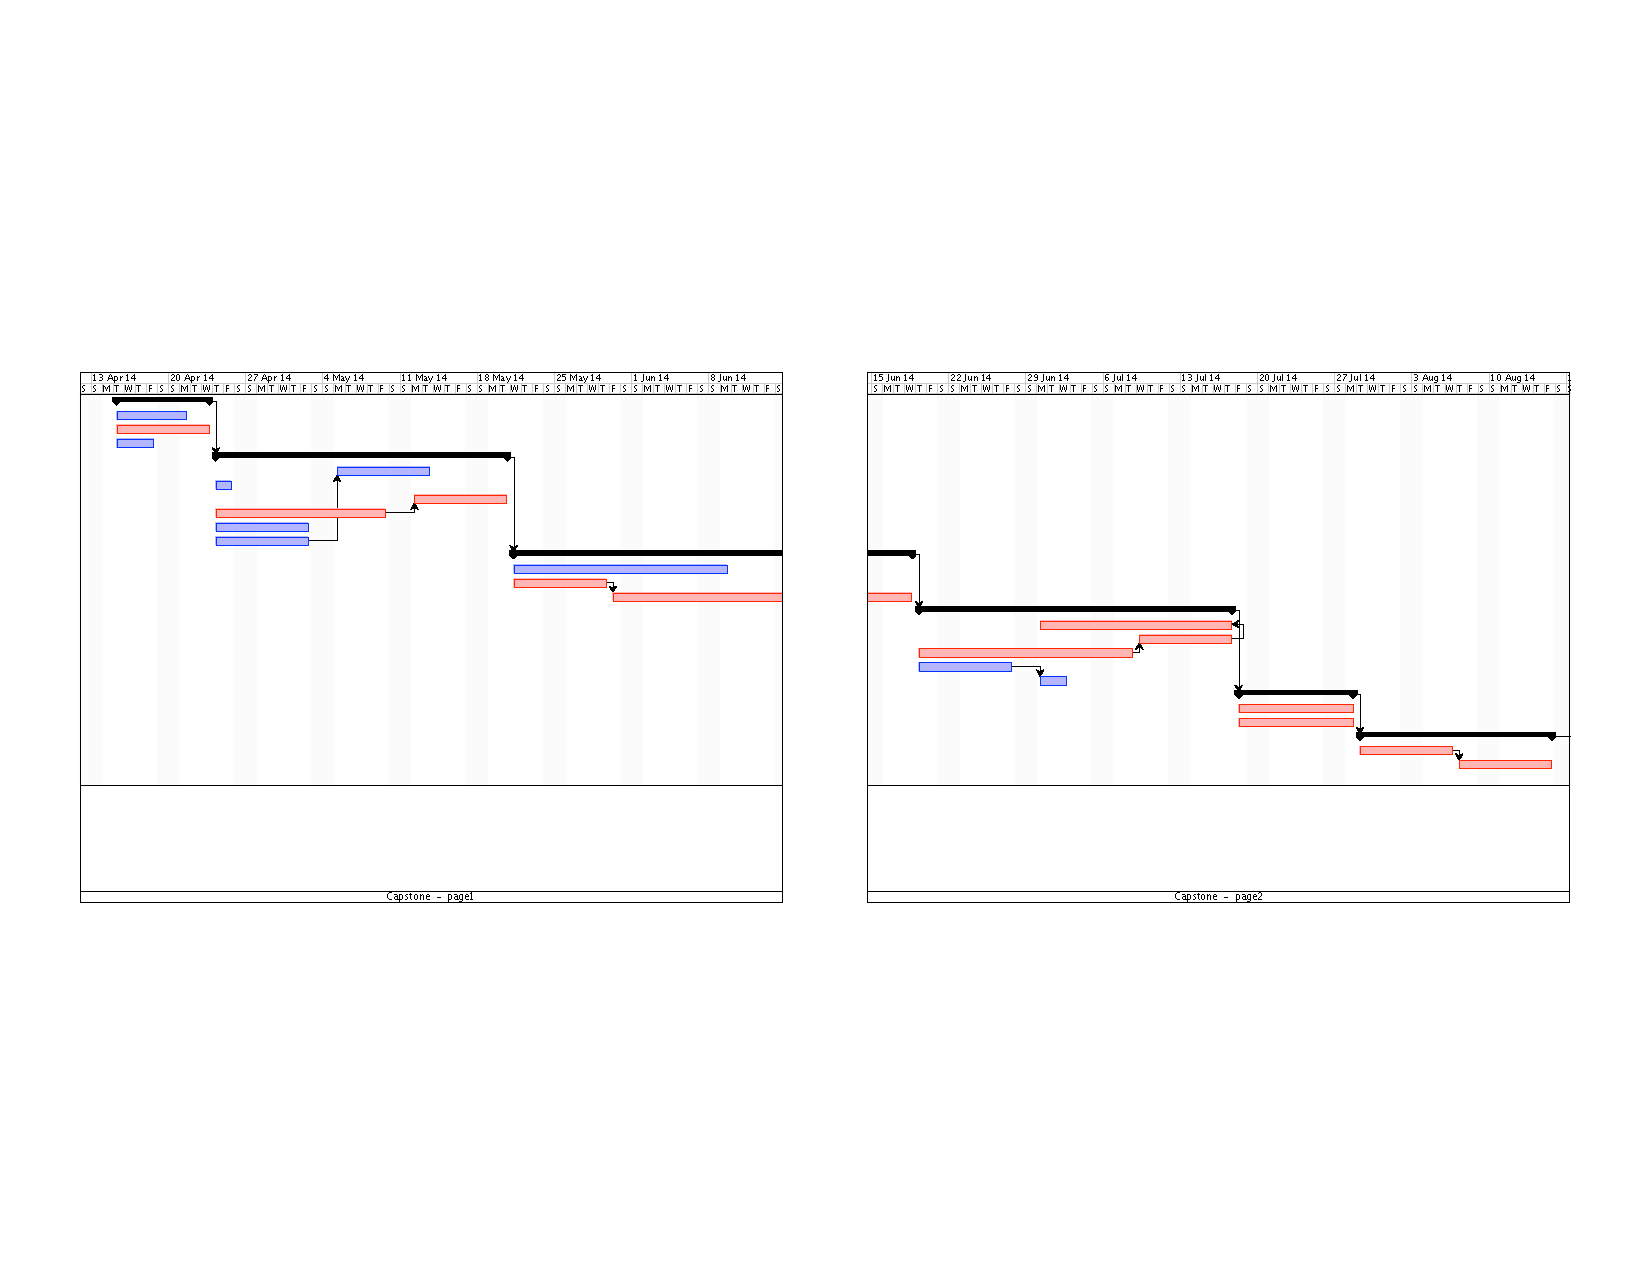
\includegraphics[width=.9\textheight, angle=90]{ganttChart}
\label{default}
\end{center}
\end{figure}


\section*{Hazard Assessment}

The dangers from any of our proposed solutions is very minor. There is a slight choking hazard depending on the final size of the blocks, as well as the ability for the device to emit small sparks from the contacts. However, the electrical hazard is very minor on battery power and is unlikely to shock a human or cause a fire.

\section*{Conclusion}

This document has presented the overall progress of our logic block puzzle device. Our current proposed solution should teach children the basics of digital logic, be suitable for a classroom environment, not endanger anyone using it, and get children interested in science, math, and computers.




\bibliographystyle{ieeetr}
\bibliography{bib}

\end{document}